% !TEX root = review.tex

Pesudopotential methods have $2$ major classes: the empirical ones
and the \textit{ab initio} ones.

\subsubsection{Hamann--Schlüte--Chiang}

\subsubsection{Kerker}

Kerker directly assumed that the pseudo-radial-wave-function is
\begin{equation}
	\chi_l (r) =
	\begin{cases}
		\mathcal{G}_l = r \mathcal{R}_l (r) & r \geq R_c (l), \\
		r^{l+1} f(r)                        & r \leq R_c (l),
	\end{cases}
\end{equation}
where $\mathcal{R}_l$ is the all-electron radial-wave-function,
$R_l = r^l f(r)$ behave like $r^l$ for small $r$ and decays rapidly for $r > R_c$.
In the paper, Kerker chose $f(r)$ to be $\exp( p(r) )$ where
\begin{equation}
	p(r) =  \alpha r^4 + \beta r^3 + \gamma r^2 + \delta.
\end{equation}
Then it is easy to derive
\begin{align}
	\ln \bigg( \frac{ \chi_l(R_c) }{ R_c^{l+1} } \bigg)
	 & = p(R_c), \label{eq:kerker0}                            \\
	R_c \frac{ \chi_l'(R_c) }{ \chi_l(R_c) }
	 & = l + 1 + R_c p'(R_c), \label{eq:kerker1}               \\
	R_c^2 p''(R_c)
	 & = R_c^2 V_l^\text{scr} (R_c) + (l + 1)^2 - R_c^2 \bigg(
	\epsilon_l + \frac{ \chi_l'(R_c) }{ \chi_l(R_c) }
	\bigg)^2, \label{eq:kerker-pp}
\end{align}
where $\chi_l (r) = r R_l$. Then apply norm-conserving condition,
\begin{equation}
	A = \int_{0}^{R_c} \abs{\mathcal{G}_l}^2 \, dr = \int_{0}^{r_c} \abs{\chi_l}^2 \, dr = I,
\end{equation}
that is, equivalently,
\begin{equation}\label{eq:cond1}
	2\delta + \ln I = \ln A.
\end{equation}
Combine $\eqref{eq:cond1}$ together with $3$ other conditions,
\begin{align}
	\chi_l (R_c)   & = \mathcal{G}_l (R_c),   \\
	\chi_l' (R_c)  & = \mathcal{G}_l' (R_c),  \\
	\chi_l'' (R_c) & = \mathcal{G}_l'' (R_c),
\end{align}
we can derive $\alpha$, $\beta$, $\gamma$ and $\delta$.
From $\eqref{eq:kerker-pp}$ the screened pesudopotential is given by
\begin{align}
	V_l^\text{scr} (r) & =
	\begin{cases}
		\mathcal{V} (r)               & r \geq R_c, \\
		\epsilon_l + \frac{ 2(l+1) }{ r } p'(r)
		+ \big(p'(r) \big)^2 + p''(r) & r \leq R_c,
	\end{cases}
\end{align}
where $\mathcal{V}$ is the all-electron potential, $\epsilon_l$ is the
eigenvalue of pesudo-wave-function as well as all-electron wave-function.
The result for $r \le R_c$ is
\begin{equation}
	V_l^\text{scr} (r) = \epsilon_l + \lambda (2 l + 2 + \lambda r^2) + 12 \alpha r^2 + 6 \beta r + 2 \gamma,
\end{equation}
where $\lambda = 4 \alpha r^2 + 3 \beta r + 2 \gamma$.

Troullier \emph{et. al.} generalized Kerker's method by simply increase
the order of $p (r)$.\cite{troullier1990straightforward}
This will be talked in section \ref{sssec:troullier}.
From Fig. \ref{fig:kerkerfig1} we can see the $3d$ all-electron wave-function is
already nodeless because there are no $d$ states in the core.
So the norm-conserving condition does not have much benefits.
This is the basis of the problem Vanderbilt\cite{Vanderbilt:1990is} will deal with, will be discussed in section \ref{sssec:us}.

\begin{figure}[H]
	\centering
	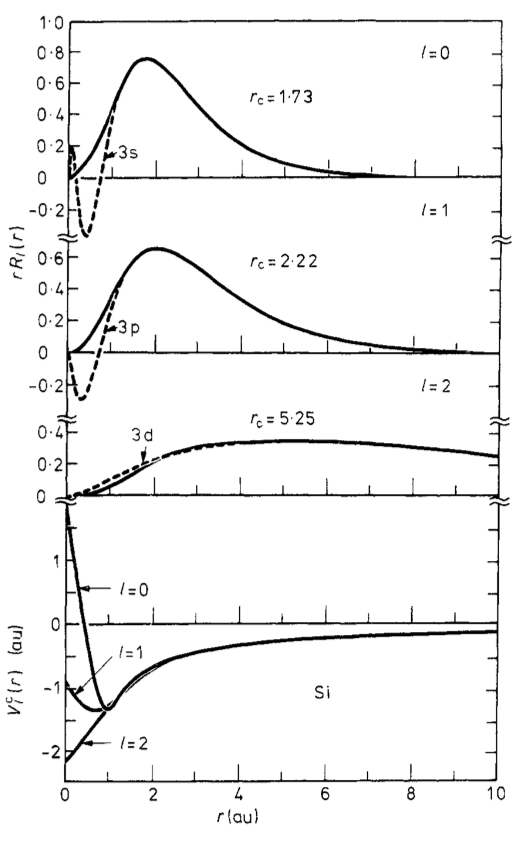
\includegraphics[height=0.5\textheight]{images/kerkerfig1}
	\caption{All-electron wave-function and pesudo-wave-function for
		\ce{Mo} $5s^1 4d^5 5p^0$ and core pesudopotential.\cite{Kerker:1980cs}}
	\label{fig:kerkerfig1}
\end{figure}














